\documentclass{article}
\usepackage{physics}
\usepackage{graphicx}
\usepackage{caption}
\usepackage{amsmath}
\usepackage{bm}
\usepackage{framed}
\usepackage{authblk}
\usepackage{empheq}
\usepackage{amsfonts}
\usepackage{esint}
\usepackage[makeroom]{cancel}
\usepackage{dsfont}
\usepackage{centernot}
\usepackage{mathtools}
\usepackage{bigints}
\usepackage{amsthm}
\theoremstyle{definition}
\newtheorem{defn}{Definition}[section]
\newtheorem{prop}{Proposition}[section]
\newtheorem{rmk}{Remark}[section]
\newtheorem{thm}{Theorem}[section]
\newtheorem{exmp}{Example}[section]
\newtheorem{prob}{Problem}[section]
\newtheorem{sln}{Solution}[section]
\newtheorem*{prob*}{Problem}
\newtheorem{exer}{Exercise}[section]
\newtheorem*{exer*}{Exercise}
\newtheorem*{sln*}{Solution}
\usepackage{empheq}
\usepackage{tensor}
\usepackage{xcolor}
%\definecolor{colby}{rgb}{0.0, 0.0, 0.5}
\definecolor{MIT}{RGB}{163, 31, 52}
\usepackage[pdftex]{hyperref}
%\hypersetup{colorlinks,urlcolor=colby}
\hypersetup{colorlinks,linkcolor={MIT},citecolor={MIT},urlcolor={MIT}}  



\newcommand*\widefbox[1]{\fbox{\hspace{2em}#1\hspace{2em}}}

\newcommand{\p}{\partial}
\newcommand{\R}{\mathbb{R}}
\newcommand{\C}{\mathbb{C}}
\newcommand{\lag}{\mathcal{L}}
\newcommand{\nn}{\nonumber}
\newcommand{\ham}{\mathcal{H}}
\newcommand{\M}{\mathcal{M}}
\newcommand{\I}{\mathcal{I}}
\newcommand{\K}{\mathcal{K}}
\newcommand{\F}{\mathcal{F}}
\newcommand{\w}{\omega}
\newcommand{\lam}{\lambda}
\newcommand{\al}{\alpha}
\newcommand{\be}{\beta}
\newcommand{\x}{\xi}

\newcommand{\G}{\mathcal{G}}

\newcommand{\f}[2]{\frac{#1}{#2}}

\newcommand{\ift}{\infty}

\newcommand{\lp}{\left(}
\newcommand{\rp}{\right)}

\newcommand{\lb}{\left[}
\newcommand{\rb}{\right]}

\newcommand{\lc}{\left\{}
\newcommand{\rc}{\right\}}


\newcommand{\V}{\mathbf{V}}
\newcommand{\U}{\mathcal{U}}
\newcommand{\Id}{\mathcal{I}}
\newcommand{\D}{\mathcal{D}}
\newcommand{\Z}{\mathcal{Z}}

%\setcounter{chapter}{-1}






\usepackage{subfig}
\usepackage{listings}
\captionsetup[lstlisting]{margin=0cm,format=hang,font=small,format=plain,labelfont={bf,up},textfont={it}}
\renewcommand*{\lstlistingname}{Code \textcolor{violet}{\textsl{Mathematica}}}
\definecolor{gris245}{RGB}{245,245,245}
\definecolor{olive}{RGB}{50,140,50}
\definecolor{brun}{RGB}{175,100,80}

%\hypersetup{colorlinks,urlcolor=colby}
\lstset{
	tabsize=4,
	frame=single,
	language=mathematica,
	basicstyle=\scriptsize\ttfamily,
	keywordstyle=\color{black},
	backgroundcolor=\color{gris245},
	commentstyle=\color{gray},
	showstringspaces=false,
	emph={
		r1,
		r2,
		epsilon,epsilon_,
		Newton,Newton_
	},emphstyle={\color{olive}},
	emph={[2]
		L,
		CouleurCourbe,
		PotentielEffectif,
		IdCourbe,
		Courbe
	},emphstyle={[2]\color{blue}},
	emph={[3]r,r_,n,n_},emphstyle={[3]\color{magenta}}
}


\begin{document}
	

\begin{center}
	\Large{Some Magnetic Traps for Neutral Atoms \\
	\& The Majorana Spin-flip for $J=1/2$.}
\end{center}	
	
\begin{center}
	\large{Huan Q. Bui}
\end{center}

\begin{center}
	\today
\end{center}



\section{Mathematica Notebook}
The Mathematica notebook which contains some calculations and sketches can be downloaded via this \href{https://raw.githubusercontent.com/huanium/huanium/master/MIT PhD/BUI_AtomicPhysics/mathematica/magnetic-traps.nb}{link}. Right-click and ``Save" to save the notebook to your computer. 


\section{Zeeman Effect \& Earnshaw's Theorem}



\section{Quadrupole trap (anti-Helmholtz)}

This section on the quadrupole trap and the next section on the TOP trap follow \cite{perez2013does}.

\subsection{Calculation}


In this configuration, there are two coils of radius $a$ placed at distance $2b$ apart. Running through the coils are equal and opposite currents $I$ and $-I$, respectively. Here, we set $I = NI_0$ where $N$ is the number of coils and $I_0$ is the current going through each coil (or equivalently through all the coils).

\begin{figure}[!htb]
	\centering
	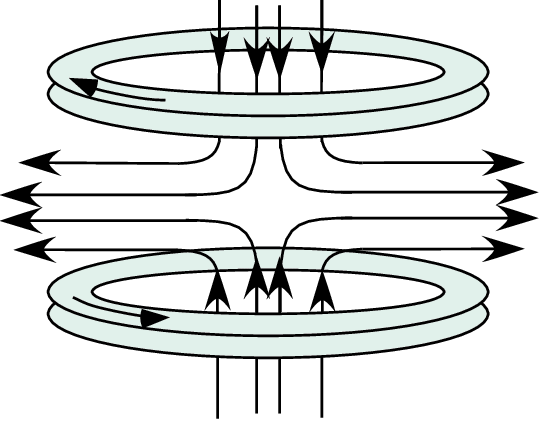
\includegraphics[width=0.6\textwidth]{antiHelmholtz.png}
	\caption{From \cite{maruyama2003optical}}
\end{figure}

To calculate the magnetic field for one coil, we can use Biot-Savart law because the current is constant. We will integrate along the closed loop $C$ defined by the coil. The relative position between the point $\mathbf{r}$ and the point $\vec{l}$ on the wire is given by $\vec{r}' = \vec{r} - \vec{l}$
\begin{equation*}
\vec{B}(\vec{r}) = \f{\mu_0 I}{4\pi} \int_C \f{d\vec{l} \times \vec{r}'}{ |{\vec{r}'}|^3} = \f{\mu_0 I}{4\pi} \int_C \f{d\vec{l} \times (\vec{r} - \vec{l})}{|{\vec{r} - \vec{l}}|^3}.  
\end{equation*}
We now make the approximation $|\vec{r}| \ll \vec{l}$ (i.e., we're interested in points far from the coil). With this we have the following expansion\footnote{a more accurate expansion will be presented in the section on the Ioffe-Pritchard trap. For our purposes in this section, it suffices to not include the term $-3|\vec{r}|^2/2|\vec{l}|^2$}
\begin{equation*}
\f{1}{|\vec{r} - \vec{l}|^3} \approx \f{1}{|\vec{l}|^3} + \f{3 \vec{r}\cdot \vec{l}}{|\vec{l}|^5} + \dots
\end{equation*}
Plugging this back in for $\vec{B}(\vec{r})$ we find 
\begin{equation*}
\vec{B}(\vec{r}) \approx \f{\mu_0 I}{4\pi}\int_C d\vec{l}\times \f{\vec{r} - \vec{l}}{|\vec{l}|^3} + \f{3\mu_0 I}{4\pi} \int_C d\vec{l} \times (\vec{r} - \vec{l}) \f{\vec{r}\cdot \vec{l}}{|\vec{l}|^5}.
\end{equation*}
Suppose that the center of the coil is at $+d$ from the $XY$ plane. Going into cylindrical coordinates, we have
\begin{equation*}
\vec{l} = a\cos\theta\hat{x} + a\sin\theta\hat{y} + d\hat{z}
\end{equation*}
from which we find 
\begin{equation*}
d\vec{l} = -a\sin\theta d\theta\hat{x} + a\cos\theta d\theta \hat{y}
\end{equation*}
So, we have
\begin{equation*}
d\vec{l} \times (\vec{r} - \vec{l}) = (-a\sin\theta, a\cos\theta,0)\times(x-a\cos\theta,y-a\sin\theta,z-d)
\end{equation*}
and 
\begin{equation*}
\vec{r}\cdot \vec{l} = xa\cos\theta + ya\sin\theta + za.
\end{equation*}
So, we have
\begin{equation*}
\f{\mu_0 I}{4\pi}\int_C d\vec{l}\times \f{\vec{r} - \vec{l}}{|\vec{l}|^3} = \f{\mu_0 I }{4\pi} \f{2a^2 \pi}{(d^2 + a^2)^{3/2}} \hat{z} = \f{\mu_0 I a^2}{2(d^2 + a^2)^{3/2}} \hat{z}.
\end{equation*}
and 
\begin{align*}
&\f{3\mu_0 I }{4\pi}\int_C d\vec{l}\times (\vec{r} - \vec{l}) \f{\vec{r}\cdot \vec{l}}{|\vec{l}|^5}\\ 
=\,\, &\f{3\mu_0 Ia^2}{4(d^2+a^2)^{5/2}} \left(- x(d-z)\hat{x}  - y (d-z)\hat{y} -  (x^2 + y^2 - 2dz)\hat{z}\right).
\end{align*}
Keeping only the linear terms and combining everything, we find the total field:
\begin{align*}
\vec{B}(\vec{r}) &= \f{\mu_0 I a^2}{2(d^2 + a^2)^{3/2}} \hat{z} + \f{3\mu_0 Ia^2}{4(d^2+a^2)^{5/2}} \left(- xd\hat{x}  -  y d\hat{y} - 2dz\hat{z}\right)\\
&= \f{\mu_0 I a^2}{2(d^2 + a^2)^{3/2}} \hat{z} + \f{3\mu_0 Ia^2 d}{2(d^2+a^2)^{5/2}} \left(- \f{x}{2}\hat{x}  -  \f{y}{2}\hat{y} - z\hat{z}\right).
\end{align*}






In the anti-Helmholtz configuration, we have two coils of radius $a$ placed a distance $2b$ apart from each other. When summing the two fields to get the total field, the first term cancels. So we get
\begin{equation*}
\vec{B}_\text{tot}(\vec{r}) = \vec{B}_{+b}(\vec{r}) + \vec{B}_{-b}(\vec{r}) = -\f{3\mu_0 I a^2 b}{2(a^2 + b^2)^{5/2}}\left( x,y,-2z \right) \equiv B_0 (x,y,-2z).
\end{equation*}
The field strength is given by 
\begin{equation*}
\abs{B(\vec{r})} = B_0 \sqrt{x^2 + y^2 + 4z^2}.
\end{equation*}

We notice that this trap is not harmonic. Further, there is a zero minimum of the magnetic field. When particles reach the zero minimum, the Zeeman shifts are reduced, leading to a loss of particles in the trap. The escape mechanism is called the Majorana spin-flip transition which we will discuss later. 


\subsection{Trap parameters}

\subsection{Simulation}


The quadrupole trap is the simplest magnetic trap configuration. The MATLAB code for this simulation is included below the figures. The code is perhaps not the most efficient way to do things, but this simulation is simple enough that we won't worry about such things for now. 


\begin{figure}[!htb]
	\centering
	\begin{minipage}{.33\textwidth}
		\centering
		\includegraphics[width=\linewidth]{sim-figs/quad-1.eps}
	\end{minipage}%
	\begin{minipage}{.33\textwidth}
		\centering
		\includegraphics[width=\linewidth]{sim-figs/quad-2.eps}
	\end{minipage}%
	\begin{minipage}{.33\textwidth}
		\centering
		\includegraphics[width=\linewidth]{sim-figs/quad-3.eps}
	\end{minipage}%
\end{figure}


\begin{lstlisting}
% Author: Huan Q. Bui
% Date: August 10, 2021

% SIMULATE Anti-Helmholtz magnetic field

clear

mu0 = 4*pi*10^(-7);
I = 10; % current in each coil, in Amperes
N = 16; % winding number
a = 0.2; % coil radius, in m
b = 0.15; % 1/2 distance between coils, in m
C = 3*mu0*I*a^2*b/(2*(a^2 + b^2)^(5/2)); % constant

x_bound = 1;
y_bound = 1;
z_bound = 1;
spacing = 0.2;

x = -x_bound:spacing:x_bound;
y = -y_bound:spacing:y_bound;
z = -z_bound:spacing:z_bound;

[X,Y,Z] = meshgrid(x,y,z);

% magnetic fields formula
% Bfield = @(x,y,z) [C.*x C.*y -2*C.*z]; 
% Bfield_XZ = @(x,z) [C.*x -2*C.*z];

h = figure(1)

% magnetic field in XZ plane
subplot(3,1,1)
quiver(X,Z,C.*X,-2*C.*Z);
xlabel('X (m)')
ylabel('Z (m)')
title('Field in XZ plane, Y=0')
xlim([-x_bound x_bound])
ylim([-z_bound z_bound])


subplot(3,1,2)
% magnetic field in YZ plane
quiver(Y,Z,C.*Y,-2*C.*Z);
xlabel('Y (m)')
ylabel('Z (m)')
title('Field in YZ plane, X=0')
xlim([-y_bound y_bound])
ylim([-z_bound z_bound])

subplot(3,1,3)
% magnetic field in XY plane
quiver(X,Y,C.*X,C.*Y);
xlabel('X (m)')
ylabel('Y (m)')
title('Field in XY plane, Z=0')
xlim([-x_bound x_bound])
ylim([-y_bound y_bound])


% Magnetic field strengths in 2D
g = figure(2)

subplot(3,1,1)
[X_XZ,Z_XZ] = meshgrid(x,z);
B_strength_XZ = sqrt((C.*X_XZ).^2  + (-2*C.*Z_XZ).^2);
surfc(X_XZ,Z_XZ,B_strength_XZ,'LineStyle' ,'none');
view(2)
xlabel('X (m)')
ylabel('Z (m)')
title('Field strength (T) in XZ, Y=0')

subplot(3,1,2)
[Y_YZ,Z_YZ] = meshgrid(y,z);
B_strength_YZ = sqrt((C.*Y_YZ).^2  + (-2*C.*Z_YZ).^2);
surfc(Y_YZ,Z_YZ,B_strength_YZ,'LineStyle' ,'none');
view(2)
xlabel('Y (m)')
ylabel('Z (m)')
title('Field strength (T) in YZ, X=0')

subplot(3,1,3)
[X_XY,Y_XY] = meshgrid(x,y);
B_strength_XY = sqrt((C.*X_XY).^2  + (-2*C.*Y_XY).^2);
surfc(X_XY,Y_XY,B_strength_XY,'LineStyle' ,'none');
view(2)
xlabel('X (m)')
ylabel('Y (m)')
title('Field strength (T) in XY, Z=0')

% magnetic field strengths in 1D
k = figure(3)
% X=0,Y=0
subplot(3,1,1)
plot(z,abs(-2*C.*z))
xlabel('Z (m)')
ylabel('B (T)')
title('Field strength in Z')
% Y=0,Z=0
subplot(3,1,2)
plot(x, abs(C.*x))
xlabel('X (m)')
ylabel('B (T)')
title('Field strength in X')
% X=0,Z=0
subplot(3,1,3)
plot(y, abs(C.*y))
xlabel('Y (m)')
ylabel('B (T)')
title('Field strength in Y')

\end{lstlisting}



\newpage

\section{TOP trap}


\subsection{Calculation}

As will be discussed later, the quadrupole or anti-Helmholtz trap suffers from the ``Majorna spin-flip problem'' which occurs due to the presence of a zero-magnetic field point in the trap. To overcome this issue, one can add a rotating magnetic field to the existing anti-Helmholtz field so that the time-averaged magnetic field no longer has a zero at the center. This trick gives us the TOP (time orbiting potential) trap. The total field is given by 
\begin{equation*}
\vec{B}(\vec{r},t) = \vec{B}_\text{quad}(\vec{r}) + \vec{B}_b(\vec{r}) = B_0 (x,y,-2z) + B_b(\cos\Omega t, \sin\Omega t,0),
\end{equation*} 
where $\Omega$ is the angular frequency of the rotating field. \\


The field strength is given by 
\begin{equation*}
B(\vec{r},t) = \sqrt{(B_0 x + B_b\cos\Omega t)^2 + (B_0 y + B_b\sin\Omega t)^2 + 4 B_0^2 z^2 }
\end{equation*}

\begin{figure}[!htb]
	\centering
	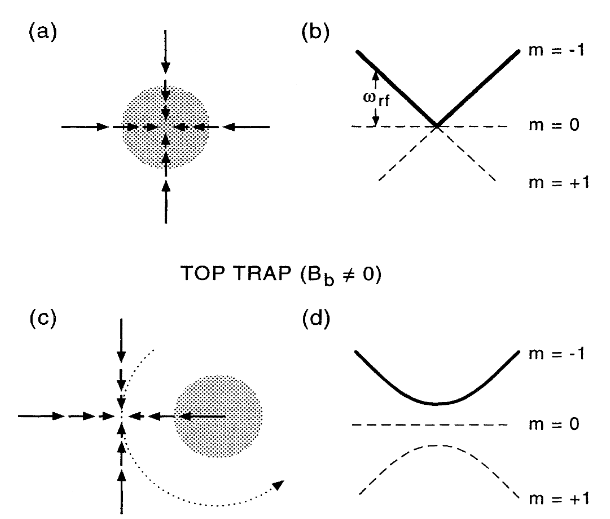
\includegraphics[width=0.6\textwidth]{TOP_trap.png}
	\caption{From \cite{PhysRevLett.74.3352}. By rotating the trap in the $XY$ plane fast enough, the atoms see a time-averaged trap that is not only quadratic (harmonic) but also has no zero minimum when $B_b \neq 0$. We note, however, that the harmonic potential is anisotropic: there is stronger confinement in the $z$-direction.}
	\label{fig:cornell}
\end{figure}

For this trap to work $\Omega$ can't be too small or too large. $\Omega$ must be larger than the oscillation frequency of the trapped particles (which is on the order of $100$ Hz) so that the particles feel an effective time-averaged magnetic field. $\Omega$ should also be smaller than the frequency associated with the transition between two adjacent internal quantum states (which is on the order of $1$ MHz) in order to prevent particle losses due to Majorana spin-flips. \\


We are interested in dynamics near the center of the trap, so we can make the approximation $r = \sqrt{x^2 + y^2 + z^2} \ll a$, under which 
\begin{equation*}
B(\vec{r},t)\approx B_b + \f{B_0^2}{2B_b^2} (x^2 + y^2 + 4z^2) + \f{B_0}{B_b}(x\cos\Omega t+ y\sin\Omega t) - \f{B_0^2}{2B_b^2}(x\cos\Omega t + y\sin\Omega t)^2.
\end{equation*}
The time-averaged magnetic field strength is thus, by inspection,
\begin{align*}
\langle B \rangle 
&= B_b  + \f{B_0^2}{2B_b^2} (x^2 + y^2 + 4z^2) - \f{B_0^2}{2B_b^2}\lp \f{x^2}{2} + \f{y^2}{2}\rp\\ &= B_b + \f{B_0^2}{4B_b}(x^2 + y^2 + 8z^2).
\end{align*}


\subsection{Trap parameters}
Here we want to calculate the trapping frequencies for the trap. Recall that the energy of a magnetic dipole moment $\mu$ acted by an external magnetic field $B$ is given by 
\begin{equation*}
E = -\mu |B|,
\end{equation*}
where $\mu \sim g_F m_F \mu_B$ (more explicit expressions for $\vec{\mu}$ which involves the spin $s$ and orbital $l$ $g$-factors can be found elsewhere).\\ 

Assuming that the energy goes like the energy for harmonic oscillation. Consider the $x$-direction with $y=z=0$ and ignoring the offset, we find
\begin{equation*}
E \sim \f{1}{2}m_\text{atom} \omega_x^2 x^2 = -\mu B = -\mu \f{B_0^2}{4B_b}x^2.
\end{equation*}
This gives
\begin{equation*}
\omega_x = \sqrt{\f{-\mu B_0^2}{2B_b m_\text{atom}}}.
\end{equation*}
By symmetry,
\begin{equation*}
\omega_y = \sqrt{\f{-\mu B_0^2}{2B_b m_\text{atom}}}
\end{equation*}
Similarly, for $z$:
\begin{equation*}
\omega_z = \sqrt{\f{-4\mu B_0^2}{B_b m_\text{atom}}}.
\end{equation*}
The aspect ratio is given by 
\begin{equation*}
\Lambda = \f{\omega_\rho}{\omega_z} = \f{\omega_x}{\omega_z} = {\f{1}{2\sqrt{2}}}.
\end{equation*}


We see that this trap works for $\mu < 0$, implying that the states are low-field seeking (so that $E = -\mu |B|$ is minimized). 

\subsection{Simulation}


The magnetic field at any given time (or instantaneous magnetic field) is simply the quadrupole magnetic field plus some shift in the $XY$ plane (as shown in Figure \ref{fig:cornell}), so we don't have to reproduce it here. The simulation only shows the time-averaged field. Once again, the (probably inefficient) MATLAB code is attached below the figures.




\begin{figure}[!htb]
	\centering
	\begin{minipage}{.49\textwidth}
		\centering
		\includegraphics[width=\linewidth]{sim-figs/TOP-1.eps}
	\end{minipage}%
	\begin{minipage}{.49\textwidth}
		\centering
		\includegraphics[width=\linewidth]{sim-figs/TOP-2.eps}
	\end{minipage}%
\end{figure}



\begin{lstlisting}
% Author: Huan Q. Bui
% Date: August 10, 2021

% SIMULATE TOP magnetic trap

clear

mu0 = 4*pi*10^(-7);
I = 1; % current in each coil, in Amperes
N = 16; % winding number
a = 0.2; % coil radius, in m
b = 0.15; % 1/2 distance between coils, in m
C = 3*mu0*I*a^2*b/(2*(a^2 + b^2)^(5/2)); % constant
B = 2*C;

x_bound = 10;
y_bound = 10;
z_bound = 10;
spacing = 0.1;

x = -x_bound:spacing:x_bound;
y = -y_bound:spacing:y_bound;
z = -z_bound:spacing:z_bound;

[X,Y,Z] = meshgrid(x,y,z);

% field strength formula:
% Bstrength = B + (C^2/(4*B))*(x^2 + y^2 + 8z^2);


% Magnetic field strengths in 2D
g = figure(1)

subplot(3,1,1)
[X_XZ,Z_XZ] = meshgrid(x,z);
B_strength_XZ = B + (C^2/(4*B))*(X_XZ.^2 + 8.*Z_XZ.^2);
surfc(X_XZ,Z_XZ,B_strength_XZ,'LineStyle' ,'none');
view(2)
xlabel('X (m)')
ylabel('Z (m)')
title('Field strength (T) in XZ, Y=0')

subplot(3,1,2)
[Y_YZ,Z_YZ] = meshgrid(y,z);
B_strength_YZ = B + (C^2/(4*B))*(Y_YZ.^2 + 8.*Z_YZ.^2);
surfc(Y_YZ,Z_YZ,B_strength_YZ,'LineStyle' ,'none');
view(2)
xlabel('Y (m)')
ylabel('Z (m)')
title('Field strength (T) in YZ, X=0')

subplot(3,1,3)
[X_XY,Y_XY] = meshgrid(x,y);
B_strength_XY = B + (C^2/(4*B))*(X_XY.^2 + Y_XY.^2);
surfc(X_XY,Y_XY,B_strength_XY,'LineStyle' ,'none');
view(2)
xlabel('X (m)')
ylabel('Y (m)')
title('Field strength (T) in XY, Z=0')

% magnetic field strengths in 1D
k = figure(2)
% X=0,Y=0
subplot(3,1,1)
plot(z,B + (C^2/(4*B)).*(8*z.^2))
xlabel('Z (m)')
ylabel('B (T)')
title('Field strength in Z')
% Y=0,Z=0
subplot(3,1,2)
plot(x, B + (C^2/(4*B)).*(x.^2))
xlabel('X (m)')
ylabel('B (T)')
title('Field strength in X')
% X=0,Z=0
subplot(3,1,3)
plot(y, B + (C^2/(4*B)).*(y.^2))
xlabel('Y (m)')
ylabel('B (T)')
title('Field strength in Y')

\end{lstlisting}



\newpage


\section{Ioffe-Pritchard traps}

This section will essentially follow \cite{allcoil} except for the calculation of the magnetic field produced by a coil. Instead of doing an expansion using Legendre polynomials and using power series expansion of the magnetic potential $\Psi$ (where $\vec{B} = \nabla \Psi$), here we simply do a series expansion for integrand of the Biot-Savart law integral and pick out terms of the same orders.  



\begin{figure}[!htb]
	\centering
	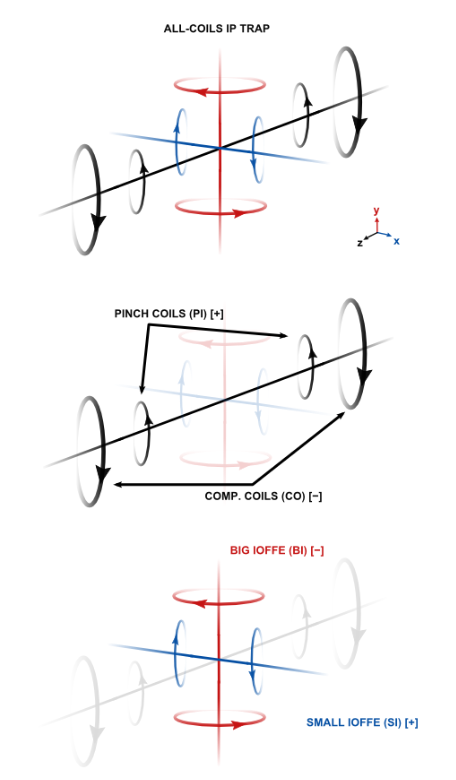
\includegraphics[width=0.75\textwidth]{all-coils.png}
	\caption{From \cite{allcoil}}
\end{figure}

\subsection{Calculation}


There are many variants of the IP trap, the simplest being one with two coils in the anti-Helmholtz configuration and four wires in the $z$-direction. The four wires are suited at the corners of a square, with the currents flowing along adjacent wires being of opposite sign. A generalization of the IP trap is often called the ``all coils Ioffe-Pritchard trap.'' The all-coil trap consists of the following set of coils:
\begin{itemize}
	\item Big Ioffe Coils (BI), anti-Helmholtz, along $z$
	\item Small Ioffe Coils (SI), anti-Helmholtz, along $x$
	\item Pinch coils (PI), Helmholtz, along $y$
	\item Compensation coils (CO), Helmholtz, along $y$, opposite current to SI.
\end{itemize}

Let us revisit the calculation we've done for Helmholtz and anti-Helmholtz coils, but now we will expand to higher orders (still assuming that $\vec{r}$ is near the origin). In particular, we will use
\begin{equation*}
\f{1}{|\vec{r} - \vec{l}|^3} \approx \f{1}{|\vec{l}|^3} 
\lb 1 -\f{3}{2}\epsilon
+ \f{15}{8}\epsilon^2 
- \f{35}{16}\epsilon^3 \rb
\end{equation*}
where
\begin{equation*}
\epsilon = \f{|\vec{r}|^2}{|\vec{l}|^2} - \f{2\vec{r}\cdot\vec{l}}{|\vec{l}|^2}.
\end{equation*}
The expansion can be obtained by following 
Eq. 3.88 of \cite{griffiths2005introduction}. We notice the difference between this expansion and the expansion that appeared in the section on the anti-Helmholtz configuration. Here, we include the term $\abs{\vec{r}}/\abs{\vec{l}}$ in $\epsilon$, so that the expansion is more accurate and match the result due to expansion in Legendre polynomials presented in \cite{allcoil}.\\


For a single coil with current $I$ placed a vertical distance $+d$ from the origin, we find the factor $|\vec{l}| = \sqrt{a^2 + d^2}$ to be constant. The field, order-by-order to third order, is thus  
\begin{equation*}
B^{(0)}(\vec{r}) = \f{\mu_0 I}{4\pi |\vec{l}|^3}\int_C d\vec{l}\times (\vec{r} - \vec{l}) = \f{1}{2}\f{\mu_0 I a^2}{(a^2 + d^2)^{3/2}} \hat{z}
\end{equation*}
\begin{align*}
B^{(1)}(\vec{r}) 
&= \f{3\mu_0 I}{4\pi |\vec{l}|^5}\int_C d\vec{l}\times (\vec{r} - \vec{l}) \lp \f{|\vec{r}|^2}{|\vec{l}|^2} - \f{2\vec{r}\cdot\vec{l}}{|\vec{l}|^2} \rp
\end{align*}
\begin{align*}
B^{(2)}(\vec{r}) 
&= \f{15\mu_0 I}{8\pi |\vec{l}|^7}\int_C d\vec{l}\times (\vec{r} - \vec{l}) \lp \f{|\vec{r}|^2}{|\vec{l}|^2} - \f{2\vec{r}\cdot\vec{l}}{|\vec{l}|^2} \rp^2
\end{align*}
\begin{align*}
B^{(3)}(\vec{r}) &= \f{35\mu_0 I}{8\pi |\vec{l}|^9}\int_C d\vec{l}\times (\vec{r} - \vec{l}) \lp \f{|\vec{r}|^2}{|\vec{l}|^2} - \f{2\vec{r}\cdot\vec{l}}{|\vec{l}|^2} \rp^3
\end{align*}
All these integrals can be done in Mathematica. The total field is found by summing the integrals. Collecting the terms order-by-order to third order (in $z$ and $\rho$) and defining $\rho^2 = x^2 + y^2$ we find that
\begin{align*}
\f{B_z(z,\rho)}{\mu_0 I} \approx &\,\,\f{1}{2}\f{a^2}{(a^2+d^2)^{3/2}} + \f{3da^2}{2(a^2+d^2)^{5/2}}z 
\\
&+ \f{3a^2(4d^2 - a^2)}{4(a^2+d^2)^{7/2}} \lp z^2 - \f{\rho^2}{2} \rp
+\f{5 a^2 d (4d^2 - 3 a^2)}{4 (a^2 + d^2)^{9/2}}\lp z^3 - \f{3 z\rho^2}{2}\rp\\
\equiv&\,\, \f{1}{2}\mathbb{F} + \mathbb{G}z + \f{1}{4}\mathbb{H}\lp z^2 - \f{\rho^2}{2} \rp + \f{1}{2} \mathbb{I}\lp z^3 - \f{3 z\rho^2}{2}\rp
\end{align*}
where 
\begin{equation*}
\mathbb{F} = \f{a^2}{(a^2+d^2)^{3/2}}, \quad 
\mathbb{G} = \f{3da^2}{2(a^2+d^2)^{5/2}}, \quad 
\mathbb{H} = \f{3a^2(4d^2-a^2)}{(a^2+d^2)^{7/2}},\quad
\mathbb{I} = \f{5 a^2 d (4 d^2-3a^2)}{2(a^2 + d^2)^{9/2}} 
\end{equation*}
are purely geometric factors. Following similar steps, we can find the field in the radial direction:
\begin{align*}
\f{B_\rho}{\mu_0 I} 
&\approx \f{\sqrt{B_x^2 + B_y^2}}{\mu_0 I} \\
&= \mathbb{G}\lp -\f{\rho}{2} \rp + \f{1}{4}\mathbb{H}(-\rho z) + \f{1}{2}\mathbb{I}\lp \f{3\rho^3}{8} - \f{3\rho z^2}{2} \rp.
\end{align*}

In these equations, we can interpret $\mathbb{F}$ as the component of the bias field, $\mathbb{G}$ of the field's gradient, and $\mathbb{H}$ of field curvature.  By symmetry, there is no field in the $\phi$ direction. 


\subsubsection{Field by Helmholtz pair}
To transform from one Helmholtz coil to the other in the Helmholtz configuration, we do the following:
\begin{equation*}
I \to I, \quad d \to -d.
\end{equation*}
With this, we can easily compute the total field.  
\begin{align*}
&B_z(z,\rho) \approx \mu_0 I \lb \mathbb{F} + \f{1}{2}\mathbb{H} \lp z^2 - \f{\rho^2}{2} \rp  \rb\\
&B_\rho(z,\rho) \approx \mu_0 I \lb \f{1}{2}\mathbb{H}(-\rho z) \rb.
\end{align*}
The other terms vanish since they are odd functions in $d$. We notice that this file only has a bias and curvature components. By letting $a=2d$ we can make  $\mathbb{H}$ vanish, producing a nearly constant field in $\hat{z}$ and almost no field in $\rho$. On the other hand, setting $a = d\sqrt{4/3}$ produces maximal $\mathbb{H}$ (maximal curvature). 



\subsubsection{Field by anti-Helmholtz pair}

To transform from one Helmholtz coil to the other in the anti-Helmholtz configuration, we do the following:
\begin{equation*}
I \to -I, \quad d \to -d.
\end{equation*}
With this, we can easily compute the total field:
\begin{align*}
&B_z(z,\rho) \approx  \mu_0 I \lb 2\mathbb{G}z + \mathbb{I}\lp z^3 - \f{3z\rho^2}{2} \rp \rb\\
&B_\rho(z,\rho) \approx \mu_0 I \lb -\mathbb{G}\rho + \mathbb{I}\lp \f{3\rho^3}{8} - \f{3\rho z^2}{2} \rp \rb
\end{align*}
where now the terms that are even in $d$ vanish. We notice that $\mathbb{I} = 0$ when $a = d\sqrt{4/3}$. Thus, configuring the field this way cancels out higher order terms. On the other hand, $\mathbb{G}$ is maximal at $a = 2d$. 




\subsubsection{Ioffe-Pritchard trap}
With the fields calculated, we now just plug everything in and find the total field in the Ioffe-Pritchard configuration. \\

We start with the big Ioffe coils (BI) in the anti-Helmholtz configuration. We will impose the condition $a_{BI} = d_{BI}\sqrt{4/3}$ so that $\mathbb{I}_{BI} = 0$. In Cartesian coordinates, this field is 
\begin{equation*}
\vec{B}_{BI}(x,y,z) = \mu_0 I_{BI} \mathbb{G}_{BI}(-x,-y,2z ).
\end{equation*}
In practice, $BI$ coils have $y$ as their symmetry axis, with current running in the opposite direction. The correct expression for the field is thus 
\begin{equation*}
\vec{B}_{BI}(x,y,z) = \mu_0 I_{BI} \mathbb{G}_{BI}(x,-2y,z).
\end{equation*}

For the small Ioffe coils, $x$ is the symmetry axis. We also impose the condition $a_{SI} = d_{SI}\sqrt{4/3}$ so that $\mathbb{I}_{SI} = 0$. Since they're also in the anti-Helmholtz configuration we have
\begin{equation*}
\vec{B}_{SI}(x,y,z) = \mu_0 I_{SI} \mathbb{G}_{SI} (2x,-y,-z).
\end{equation*}

For the pinch coils (PI) which are in the Helmholtz configuration, we find 
\begin{equation*}
\vec{B}_{PI}(x,y,z) = \mu_0 I_{PI} \lp -\f{1}{2}\mathbb{H}_{PI}xz,  -\f{1}{2}\mathbb{H}_{PI}yz, \mathbb{F}_{PI} + \f{1}{2}\mathbb{H}_{PI} \lp z^2 - \rho^2/2 \rp \rp.
\end{equation*}

Finally, we have the compensation coils (CO), which are in the Helmholtz configuration, but the current is in the opposite direction to PI's. The field is 
\begin{equation*}
\vec{B}_{CO}(x,y,z) = \mu_0 I_{CO} \lp \f{1}{2}\mathbb{H}_{CO}xz,  \f{1}{2}\mathbb{H}_{CO}yz, -\mathbb{F}_{CO} - \f{1}{2}\mathbb{H}_{CO} \lp z^2 - \rho^2/2 \rp \rp.
\end{equation*}

Adding everything up we find the full field:
\begin{align*}
\vec{B}(x,y,z) = 
&\begin{pmatrix}
0\\
0\\ 
\mu_0 I_{PI} \mathbb{F}_{PI} - \mu_0 I_{CO} \mathbb{F}_{CO} 
\end{pmatrix}
+ 
\begin{pmatrix}
(\mu_0 I_{BI}\mathbb{G}_{BI}  +2 \mu_0 I_{SI} \mathbb{G}_{SI}  )x\\
-(2\mu_0 I_{BI}\mathbb{G}_{BI} +\mu_0 I_{SI} \mathbb{G}_{SI})y\\
(\mu_0 I_{BI} \mathbb{G}_{BI} - \mu_0 I_{SI} \mathbb{G}_{SI})z
\end{pmatrix}\\
&+ \f{1}{2} \lp \mu_0 I_{PI}\mathbb{H}_{PI} -\mu_0 I_{CO}\mathbb{H}_{CO}  \rp \begin{pmatrix}
-xz\\-yz\\z^2 - \rho^2/2
\end{pmatrix}.
\end{align*}
We now add another constraint:
\begin{equation*}
\mu_0 I_{BI} \mathbb{G}_{BI} = \mu_0 I_{SI} \mathbb{G}_{SI}
\end{equation*}
so that the full field simplifies to:
\begin{align*}
\vec{B}(x,y,z) = 
\delta \begin{pmatrix}
0\\
0\\ 
1
\end{pmatrix}
+ 
\al \begin{pmatrix}
x\\
-y\\
0
\end{pmatrix}
+ \f{1}{2}\beta \begin{pmatrix}
-xz\\-yz\\z^2 - \rho^2/2
\end{pmatrix}
\end{align*}
where
\begin{align*}
&\al = 3\mu_0 I_{BI}\mathbb{G}_{BI} = 3\mu_0 I_{SI}\mathbb{G}_{SI}\\
&\beta = \mu_0 I_{PI}\mathbb{H}_{PI} -\mu_0 I_{CO}\mathbb{H}_{CO} \\
&\delta = \mu_0 I_{PI} \mathbb{F}_{PI} - \mu_0 I_{CO} \mathbb{F}_{CO} .
\end{align*}



\subsection{Trap parameters}

Just as before, we want to calculate the trapping frequencies. Following a similar approach, we find the trapping frequency in the $z$-direction by setting $x=y=0$ and calculate $|\vec{B}|$ then extract $\omega_z$:
\begin{equation*}
\f{1}{2}m_\text{atom} \omega_z^2 z^2 = g_F m_F \mu_B\f{1}{2}\beta z^2
\end{equation*}
from which we find 
\begin{equation*}
\omega_z = \sqrt{\f{ g_F m_F \mu_B \beta}{m_\text{atom}}} = \sqrt{\f{g_F m_F \mu_B\mu_0 }{m_\text{atom}}\lp I_{PI}\mathbb{H}_{PI} - I_{CO}\mathbb{H}_{CO} \rp }.
\end{equation*}
Similarly, setting $z=0$ we find the field strength to be 
\begin{align*}
|\vec{B}| &= \sqrt{\al^2 \rho^2 + \delta^2 - \f{1}{2}\delta \beta \rho^2 + \cancel{\f{1}{16}\be^2 \rho^4}}\\
&\approx \sqrt{\delta^2 + \lp  \al^2 - \f{1}{2}\delta \beta\rp\rho^2} \\
&= \delta \sqrt{1 + \lp \f{\al^2}{\delta^2} - \f{\beta}{2\delta} \rp\rho^2 }\\
&\approx \delta \lb 1 + \f{1}{2}\lp \f{\al^2}{\delta^2} - \f{\be}{2\delta} \rp \rho^2 \rb\\
&= \delta + \f{1}{2}\lp \f{\al^2}{\delta} - \f{\beta}{2} \rp \rho^2
\end{align*}
As before, we only care about the curvature part:
\begin{equation*}
\f{1}{2}m_\text{atom} \omega_\rho^2 \rho^2 = g_F m_F \mu_B \f{1}{2}\lp \f{\al^2}{\delta} - \f{\beta}{2} \rp\rho^2
\end{equation*}
which gives
\begin{align*}
\omega_\rho &= \sqrt{\f{g_F m_F \mu_B}{m_\text{atom}} \lp \f{\al^2}{\delta} - \f{\be}{2} \rp  } \\
&= \sqrt{\f{g_F m_F \mu_B \mu_0}{m_\text{atom}} \lp \f{9I_{BI}\mathbb{G}_{BI}^2}{ I_{PI} \mathbb{F}_{PI} -  I_{CO} \mathbb{F}_{CO} }  - \f{ I_{PI}\mathbb{H}_{PI} - I_{CO}\mathbb{H}_{CO}}{2} \rp }.
\end{align*}



We can put on more constraints to further simplify things. In particular, we can let $a_{CO} = 2d_{CO}$ so that $\mathbb{H}_{CO} = 0$, meaning that the compensation coils only contribute to the bias field. With this constraint, we have
\begin{equation*}
\omega_z = \sqrt{\f{g_F m_F \mu_B\mu_0 }{m_\text{atom}} I_{PI}\mathbb{H}_{PI}  }
\end{equation*}
\begin{equation*}
\omega_\rho = \sqrt{\f{g_F m_F \mu_B \mu_0}{m_\text{atom}} \lp \f{9I_{BI}\mathbb{G}_{BI}^2}{ I_{PI} \mathbb{F}_{PI} -  I_{CO} \mathbb{F}_{CO} }  - \f{ I_{PI}\mathbb{H}_{PI} }{2} \rp }.
\end{equation*}


As before, the aspect ratio can be calculated via
\begin{equation*}
\Lambda = \f{\omega_\rho}{\omega_z}.
\end{equation*}



\subsection{Simulation}
As opposed to the MATLAB code provided in \cite{allcoil}, the simulation below uses the expression for $\vec{B}$ which approximates to third order the total magnetic field near the center of the trap. The reader may refer to \cite{allcoil} for the exact simulation for the full field, evaluates the fields due to the coils exactly using numerical integration of elliptic integrals. The reader are also welcomed to compare the results generated using the approximate simulation presented here and those from the full simulation of \cite{allcoil}.\\


First, we reproduce the first simulation of \cite{allcoil} where $N = 16, \delta = 5$G, $I_{SI} 50$A, and $I_{PI}=12$A. All calculated parameters are listed below the figure. They agree well with the exact simulation provided by \cite{allcoil}. Next, without changing any parameters, we reproduce the fields in the $XY,YZ,ZX$ planes.


\begin{figure}[!htb]
	\centering
	
	\begin{minipage}{.49\textwidth}
		\centering
		\includegraphics[width=\linewidth]{sim-figs/IP-1.eps}
	\end{minipage}%
	\begin{minipage}{.49\textwidth}
		\centering
		\includegraphics[width=\linewidth]{sim-figs/IP-2.eps}
	\end{minipage}%
	\caption{Simulation with $N = 16, \delta = 5$G, $I_{SI} = 50$A, and $I_{PI}=12$A. We see the ``pencil'' like aspect ratio in the profile of $|B|$ in the $XZ$ and $YZ$ planes, signifying axial confinement. Calculated parameters shown below.}
\end{figure}


\begin{lstlisting}
-----------------------
Omega_Z: 20.4911 rad/s
Omega_Rho: 203.7857 rad/s
Aspect Ratio: 9.9451
-----------------------
delta: 5 G
alpha: 80.5921 G/cm
beta: 13.068 G/cm^2
-----------------------
J_BI: 112.6733 A
J_SI: 50 A
J_CO: 12.7507 A
J_PI: 12 A
-----------------------
a_BI: 5.2 cm
a_SI: 3.464 cm
a_CO: 5 cm
a_PI: 2.5 cm
-----------------------
d_BI: 4.5033 cm
d_SI: 2.9999 cm
d_CO: 2.5 cm
d_PI: 2.1651 cm
-----------------------
\end{lstlisting}

By modifying the parameters and removing some of the constraints, one can generate more ``interesting'' profiles shown in \cite{allcoil}. However we won't worry about that here. 



\newpage



\section{The Majorana spin-flip problem}





\newpage

\bibliography{Bui_MagTrap} 
\bibliographystyle{unsrt}	

\end{document}